% Options for packages loaded elsewhere
\PassOptionsToPackage{unicode}{hyperref}
\PassOptionsToPackage{hyphens}{url}
\PassOptionsToPackage{dvipsnames,svgnames*,x11names*}{xcolor}
%
\documentclass[
]{article}
\usepackage{lmodern}
\usepackage{amssymb,amsmath}
\usepackage{ifxetex,ifluatex}
\ifnum 0\ifxetex 1\fi\ifluatex 1\fi=0 % if pdftex
  \usepackage[T1]{fontenc}
  \usepackage[utf8]{inputenc}
  \usepackage{textcomp} % provide euro and other symbols
\else % if luatex or xetex
  \usepackage{unicode-math}
  \defaultfontfeatures{Scale=MatchLowercase}
  \defaultfontfeatures[\rmfamily]{Ligatures=TeX,Scale=1}
\fi
% Use upquote if available, for straight quotes in verbatim environments
\IfFileExists{upquote.sty}{\usepackage{upquote}}{}
\IfFileExists{microtype.sty}{% use microtype if available
  \usepackage[]{microtype}
  \UseMicrotypeSet[protrusion]{basicmath} % disable protrusion for tt fonts
}{}
\makeatletter
\@ifundefined{KOMAClassName}{% if non-KOMA class
  \IfFileExists{parskip.sty}{%
    \usepackage{parskip}
  }{% else
    \setlength{\parindent}{0pt}
    \setlength{\parskip}{6pt plus 2pt minus 1pt}}
}{% if KOMA class
  \KOMAoptions{parskip=half}}
\makeatother
\usepackage{xcolor}
\IfFileExists{xurl.sty}{\usepackage{xurl}}{} % add URL line breaks if available
\IfFileExists{bookmark.sty}{\usepackage{bookmark}}{\usepackage{hyperref}}
\hypersetup{
  colorlinks=true,
  linkcolor=blue,
  filecolor=Maroon,
  citecolor=Blue,
  urlcolor=Blue,
  pdfcreator={LaTeX via pandoc}}
\urlstyle{same} % disable monospaced font for URLs
\usepackage{graphicx}
\makeatletter
\def\maxwidth{\ifdim\Gin@nat@width>\linewidth\linewidth\else\Gin@nat@width\fi}
\def\maxheight{\ifdim\Gin@nat@height>\textheight\textheight\else\Gin@nat@height\fi}
\makeatother
% Scale images if necessary, so that they will not overflow the page
% margins by default, and it is still possible to overwrite the defaults
% using explicit options in \includegraphics[width, height, ...]{}
\setkeys{Gin}{width=\maxwidth,height=\maxheight,keepaspectratio}
% Set default figure placement to htbp
\makeatletter
\def\fps@figure{htbp}
\makeatother
\setlength{\emergencystretch}{3em} % prevent overfull lines
\providecommand{\tightlist}{%
  \setlength{\itemsep}{0pt}\setlength{\parskip}{0pt}}
\setcounter{secnumdepth}{5}

%% pandoc-fignos: required package
\usepackage{cleveref}
\newlength{\cslhangindent}
\setlength{\cslhangindent}{1.5em}
\newenvironment{cslreferences}%
  {}%
  {\par}

\author{}
\date{}

\begin{document}

\hypertarget{support-vector-machines}{%
\section{Support Vector Machines}\label{support-vector-machines}}

\hypertarget{introduction}{%
\subsection{Introduction}\label{introduction}}

Suppose that we are given a collection of data made up of samples from
two different classes, and we would like to develop an algorithm that
can distinguish between the two classes. For example, given a picture
that is either a dog or a cat, we'd like to be able to say which of the
pictures are dogs, and which are cats. For another example, we might
want to be able to distinguish ``real'' emails from ``spam.'' This type
of problem is called a \emph{classification} problem.

Typically, one approaches a classification problem by beginning with a
large set of data for which you know the classes, and you use that data
to \emph{train} an algorithm to correctly distinguish the classes for
the test cases where you already know the answer. For example, you start
with a few thousand pictures labelled ``dog'' and ``cat'' and you build
your algorithm so that it does a good job distinguishing the dogs from
the cats in this initial set of \emph{training data}. Then you apply
your algorithm to pictures that aren't labelled and rely on the
predictions you get, hoping that whatever let your algorithm distinguish
between the particular examples will generalize to allow it to correctly
classify images that aren't pre-labelled.

Because classification is such a central problem, there are many
approaches to it. We will see several of them through the course of
these lectures. We will begin with a particular classification algorithm
called ``Support Vector Machines'' (SVM) that is based on linear
algebra. The SVM algorithm is widely used in practice and has a
beautiful geometric interpretation, so it will serve as a good beginning
for later discussion of more complicated classification algorithms.

Incidentally, I'm not sure why this algorithm is called a ``machine'';
the algorithm was introduced in the paper
{[}\protect\hyperlink{ref-vapnik92}{1}{]} where it is called the
``Optimal Margin Classifier'' and as we shall see that is a much better
name for it.

\hypertarget{a-simple-example}{%
\subsection{A simple example}\label{a-simple-example}}

Let us begin our discussion with a very simple dataset (see
{[}\protect\hyperlink{ref-penguins}{2}{]} and
{[}\protect\hyperlink{ref-penguindata}{3}{]}). This data consists of
various measurements of physical characteristics of 344 penguins of 3
different species: Gentoo, Adelie, and Chinstrap. If we focus our
attention for the moment on the Adelie and Gentoo species, and plot
their body mass against their culmen depth, we obtain the following
scatterplot.

\begin{figure}
\hypertarget{fig:penguins}{%
\centering
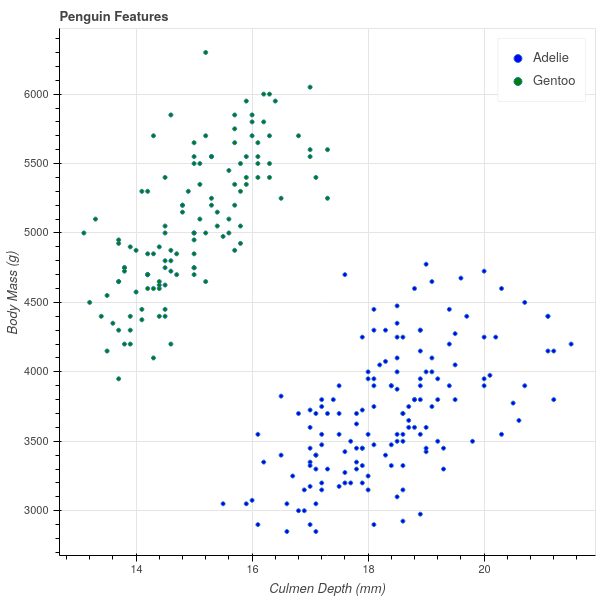
\includegraphics[width=0.5\textwidth,height=\textheight]{../img/penguins.png}
\caption{Penguin Scatterplot}\label{fig:penguins}
}
\end{figure}

Incidentally, a bird's \emph{culmen} is the upper ridge of their beak,
and the \emph{culmen depth} is a measure of the thickness of the beak.
There's a nice picture at {[}\protect\hyperlink{ref-penguindata}{3}{]}
for the penguin enthusiasts.

A striking feature of this scatter plot is that there is a clear
separation between the clusters of Adelie and Gentoo penguins. Adelie
penguins have deeper culmens and less body mass than Gentoo penguins.
These characteristics seem like they should provide a way to classify a
penguin between these two species based on these two measurements.

One way to express the separation between these two clusters is to
observe that one can draw a line on the graph with the property that all
of the Adelie penguins lie on one side of that line and all of the
Gentoo penguins lie on the other. In \cref{fig:penguinsline} I've drawn
in such a line (which I found by eyeballing the picture in
\cref{fig:penguins}). The line has the equation \[
Y = 250X+400.
\]

\begin{figure}
\hypertarget{fig:penguinsline}{%
\centering
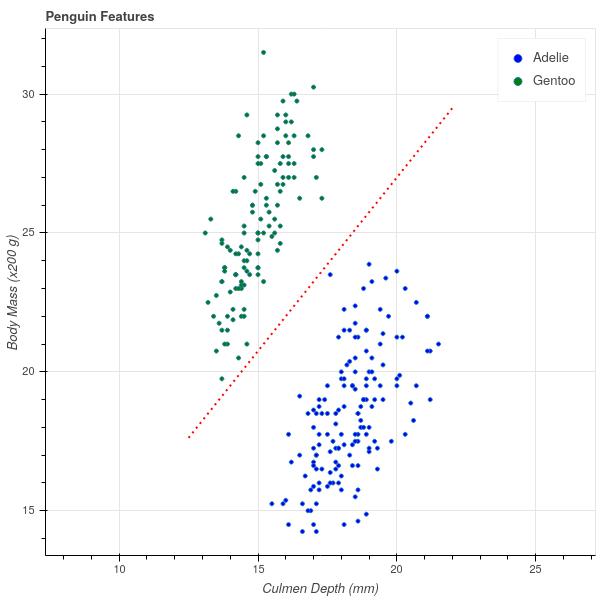
\includegraphics[width=0.5\textwidth,height=\textheight]{../img/penguins_with_line.png}
\caption{Penguins with Separating Line}\label{fig:penguinsline}
}
\end{figure}

The fact that all of the Gentoo penguins lie above this line means that,
for the Gentoo penguins, their body mass in grams is at least \(400\)
more than \(250\) times their culmen depth in mm.

\[
\mathrm{Gentoo\ mass}> 250(\mathrm{Gentoo\ culmen\ depth})+400
\]

while

\[
\mathrm{Adelie\ mass}<250(\mathrm{Adelie\ culmen\ depth})+400.
\]

Now, if we measure a penguin caught in the wild, we can compute
\(250(\mathrm{culmen\ depth})+400\) for that penguin and if this number
is greater than the penguin's mass, we say it's an Adelie; otherwise, a
Gentoo. Based on the experimental data we've collected -- the
\emph{training} data -- this seems likely to work pretty well.

\hypertarget{the-general-case}{%
\subsection{The general case}\label{the-general-case}}

To generalize this approach, let's imagine now that we have \(n\)
samples and \(k\) features (or measurements) for each sample. As before,
we can represent this data as an \(n\times k\) data matrix \(X\). In the
penguin example, our data matrix would be \(344\times 2\), with one row
for each penguin and the columns representing the mass and the culmen
depth. In addition to this numerical data, we have a classification that
assigns each row to one of two classes. Let's represent the classes by a
\(n\times 1\) vector \(Y\), where \(y_{i}=+1\) if the \(i^{th}\) sample
is in one class, and \(y_{i}=-1\) if that \(i^{th}\) sample is in the
other. Our goal is to predict \(Y\) based on \(X\) -- but unlike in
linear regression, \(Y\) takes on the values of \(\pm 1\).

In the penguin case, we were able to find a line that separated the two
classes. We can generalize this notion to higher dimensions.

\textbf{Definition:} Suppose that we have an \(n\times k\) data matrix
\(X\) and a set of labels \(Y\) that assign the \(n\) samples to one of
two classes. Then the labelled data is said to be \emph{linearly
separable} if there is a degree one polynomial \[
f(x) = f(x_1,\ldots, x_k) = a_1 x_1 + a_2 x_2 +\cdots + a_k x_k + b
\] so that \(f(x)>0\) whenever \(x=(x_1,\ldots, x_k)\) is a row of \(X\)
-- a sample -- belonging to the \(+1\) class, and \(f(x)<0\) whenever
\(x\) belongs to the \(-1\) class. A function \(f\) that satisfies this
property is called a \emph{separating hyperplane}.

In \(\mathbf{R}^{k}\), the set of points \(x\) where \(f(x)=0\) is a
hyperplane, and the regions where \(f(x)>0\) and \(f(x)<0\) are the two
``sides'' of that hyperplane. So the definition says that two sets are
linearly separable if we can find a hyperplane so that each set lies on
a different side of that hyperplane.

Our classification strategy, then, is to find a separating hyperplane
\(f\) for our training data. Then, given a point \(x\) whose class we
don't know, we can evaluate \(f(x)\) and assign \(x\) to a class
depending on whether \(f(x)>0\) or \(f(x)<0\).

This definition begs two questions about a particular dataset:

\begin{enumerate}
\def\labelenumi{\arabic{enumi}.}
\tightlist
\item
  How do we tell if the two classes are linearly separable?
\item
  If the two sets are linearly separable, there are infinitely many
  separating hyperplanes. To see this, look back at the penguin example
  and notice that we can `wiggle' the red line a little bit and it will
  still separate the two sets. Which is the `best' separating
  hyperplane?
\end{enumerate}

For the moment, we will table the first question, and \emph{assume} that
our data belongs to two classes that are linearly separable, and we will
look at one possible answer to the second question: what's the best
separating hyperplane?

\hypertarget{margins}{%
\subsection{Margins}\label{margins}}

Let's look at a simplified version of the penguin data, where we have
two linearly separable clusters of points in the plane. In
\cref{fig:penguinsimple} we show a plot of a randomly selected subset of
the penguin points, along with the line \(Y=250X+400\) that we eyeballed
earlier.

\begin{figure}
\hypertarget{fig:penguinsimple}{%
\centering
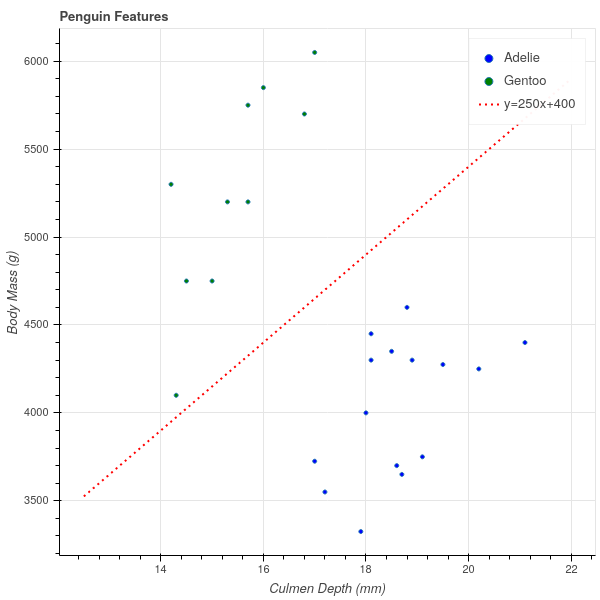
\includegraphics[width=0.5\textwidth,height=\textheight]{../img/penguinsimple.png}
\caption{A subset of penguins}\label{fig:penguinsimple}
}
\end{figure}

One way to measure how well this line separates the two clusters is to
ask how close the nearest point in each cluster is to the line. Looking
at \cref{fig:penguinsimple}, you'll notice that the line is closer to
the green (Gentoo) cluster than it is to the blue (Adelie) cluster. So,
at least as far as this subset of the data is concerned, we could get
better separation if we moved the line downwards.

Of course, we could also tilt the line by changing its slope, and
perhaps if we increased the slope a bit, that would get us better
separation as well.

In any case, this suggests that we measure the effectiveness of our line
at separating the two clusters by \emph{looking at the distance from the
line to the closest point(s) in each cluster, and trying to make those
distances as large as possible.}

The following lemma reminds us of a few facts about hyperplanes in
\(\mathbf{R}^{k}\), including how to compute the distance from a point
to a line (or to a hyperplane in higher dimensions).

\textbf{Lemma:} Let \(f(x_1,\ldots, x_k) = \sum_{i=1}^{k} a_i x_i +b\)
with not all \(a_i=0\). Let \(w=(a_1,\ldots,a_k)\) viewed as a vector in
\(\mathbf{R}^{k}\), so that if we view \(x=(x_1,\ldots, x_k)\) as a
vector we can write a vector version of \(f\): \[
f(x)=w\cdot x+b.
\]

\begin{itemize}
\tightlist
\item
  The vector \(w\) is normal vector to the hyperplane \(f(x)=0\).
  Concretely this means that if \(p\) and \(q\) are any two points in
  that hyperplane, then \(w\cdot (p-q)=0\).
\item
  Let \(p=(u_1,\ldots,u_k)\) be a point in \(\mathbf{R}^{k}\). Then the
  perpendicular distance \(D\) from \(p\) to the hyperplane \(f(x)=0\)
  is \[
  D = \frac{f(p)}{\|w\|}
  \]
\end{itemize}

\hypertarget{bibliography}{%
\section*{References}\label{bibliography}}
\addcontentsline{toc}{section}{References}

\hypertarget{refs}{}
\begin{cslreferences}
\leavevmode\hypertarget{ref-vapnik92}{}%
{[}1{]} \textsc{Boser}, B., \textsc{Guyon}, I. and \textsc{Vapnik}, V. A
training algorithm for optimal margin classifiers. In \emph{Colt '92:
Proceedings of the fifth annual workshop on computational learning
theory} (D. Haussler, ed) pp 144--52. ACM.

\leavevmode\hypertarget{ref-penguins}{}%
{[}2{]} \textsc{KB}, G., \textsc{TD}, W. and \textsc{WR}, F. (2014).
Ecological sexual dimorphism and environmental variability within a
community of antarctic penguins (genus pygoscelis). \emph{PLoS ONE}
\textbf{9(3)} --13.

\leavevmode\hypertarget{ref-penguindata}{}%
{[}3{]} \textsc{Horst}, A. Palmer penguins.Available at
\url{https://https://github.com/allisonhorst/palmerpenguins}.
\end{cslreferences}

\end{document}
